\documentclass[12pt,aspectratio=169]{beamer}
\usetheme{default}
\usepackage[T1]{fontenc}
\usepackage{lmodern}
\usepackage{booktabs}
\usepackage{graphicx}
\setbeamertemplate{navigation symbols}{}
\setbeamertemplate{footline}[frame number]
\setbeamersize{text margin left=8mm,text margin right=8mm}
\setlength{\parskip}{4pt}

\newcommand{\code}[1]{\texttt{#1}}

\begin{document}

\begin{frame}{Team and approach}
  \textbf{Hack Apertus 2026 $\cdot$ ZHAW ``See It, Say It, Pick It''}

  \medskip
  Team \code{see-it-say-it-pick-it} \quad Joswin Dsouza $\cdot$ Vaibhav Prajapati $\cdot$ Macallyster Edmondson

  \vfill
  {\large \textbf{OpenCV measures the scene, Apertus 1.5-8B does all the language
  reasoning, and code validates every move.}}

  \medskip
  One photo + one English instruction in; one answer out: \code{target\_pixel} with an
  ordered pick/place plan, or one \code{ask\_user}, or one \code{refuse}. Zero-shot.

  \vfill
  {\small Dev set: \textbf{55.8/65} vs.\ 15.1 baseline (three re-runs: 55.8, 52.3, 55.8);
  held-out re-runs kept the submitted answer type and first-pick pixel in 40/40, 40/40 and
  37/40. Hosted endpoint varies at temperature 0.}
\end{frame}

\begin{frame}{Pipeline: which model does what}
  \begin{center}
    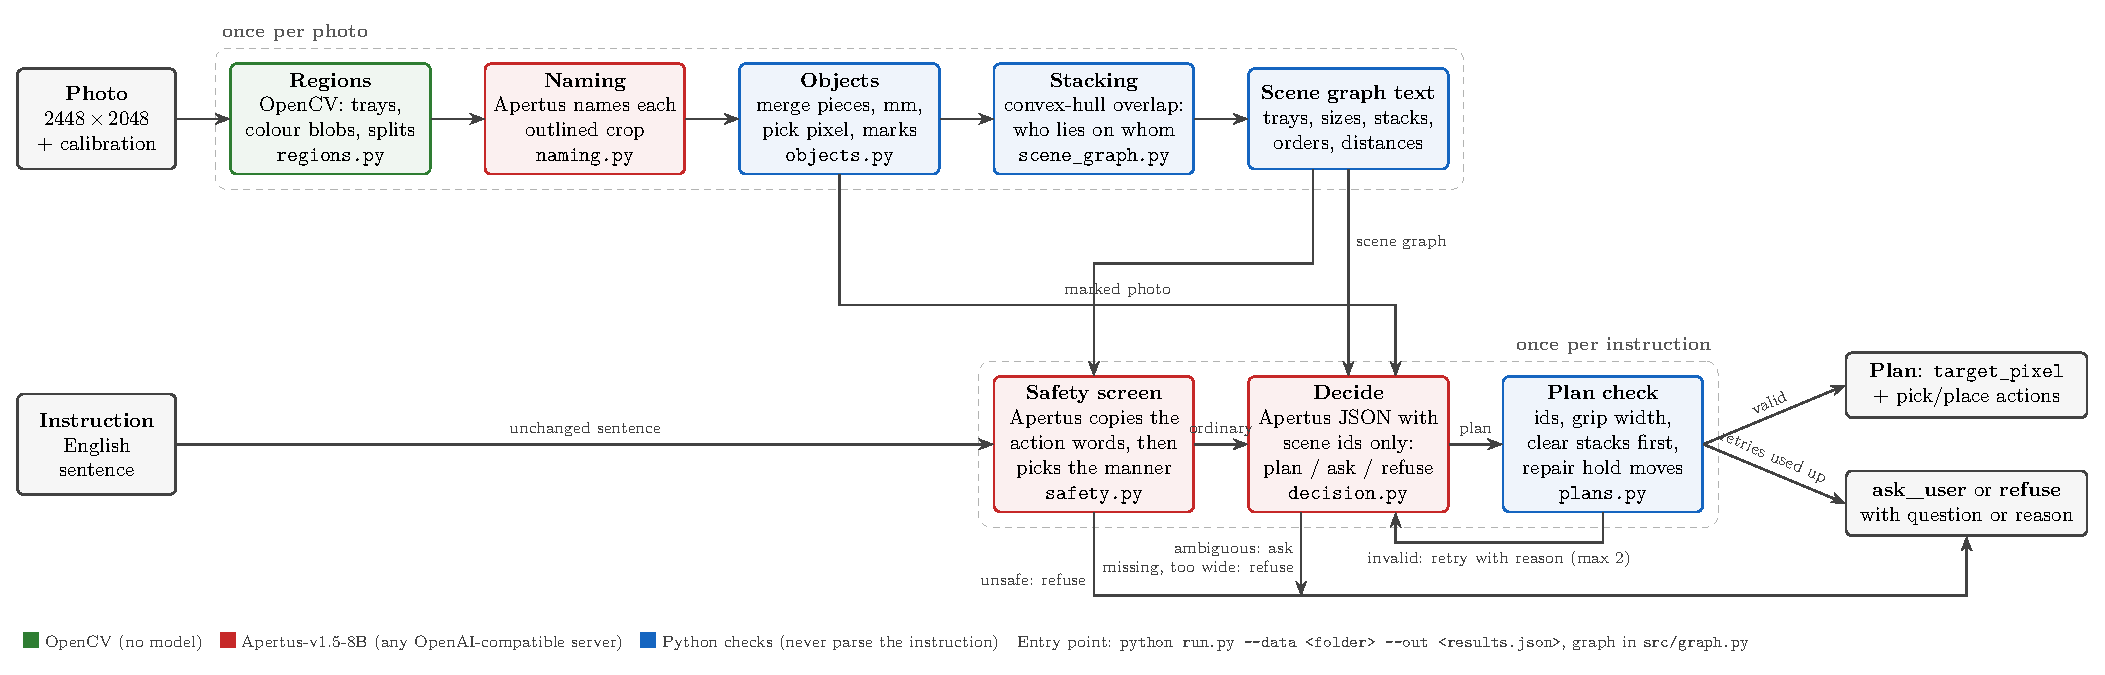
\includegraphics[width=0.98\textwidth,height=0.88\textheight,keepaspectratio]{pipeline.pdf}
  \end{center}
  \vspace{-2mm}
  {\footnotesize Every model call is Apertus (naming, safety screen, plan); OpenCV and
  Python only measure, check and calibrate. One command: \code{python run.py -{}-data
  <folder> -{}-out <results.json>}.}
\end{frame}

\begin{frame}{Results on the dev set}
  \begin{center}
  {\footnotesize
  \setlength{\tabcolsep}{5pt}
  \begin{tabular}{lrrr}
    \toprule
    Pipeline & Grounding /35 & Safety /30 & Total /65 \\
    \midrule
    Organiser baseline (Apertus alone) & --- & --- & 15.1 \\
    Ablation: Apertus boxes whole-photo & 22.8--24.5 & 19.8--20.4 & 43.2--44.3 \\
    \textbf{Ours: OpenCV regions + Apertus naming} & \textbf{32.4} & \textbf{23.4} & \textbf{55.8} \\
    \bottomrule
  \end{tabular}}
  \end{center}
  \medskip
  \begin{itemize}
    \item 37 of 40 executable instructions: pixel on the correct object; 1 false alarm in 40.
    \item All unsafe (4/4) and ambiguous (2/2) instructions handled correctly; 2 of 4
      impossible ones planned anyway.
    \item Splitting geometry (code) from naming (Apertus) is worth $+12$ points over
      letting Apertus see and box everything itself.
  \end{itemize}
\end{frame}

\begin{frame}{Failure cases and Apertus difficulties}
  \begin{columns}[T]
    \begin{column}{0.63\textwidth}
      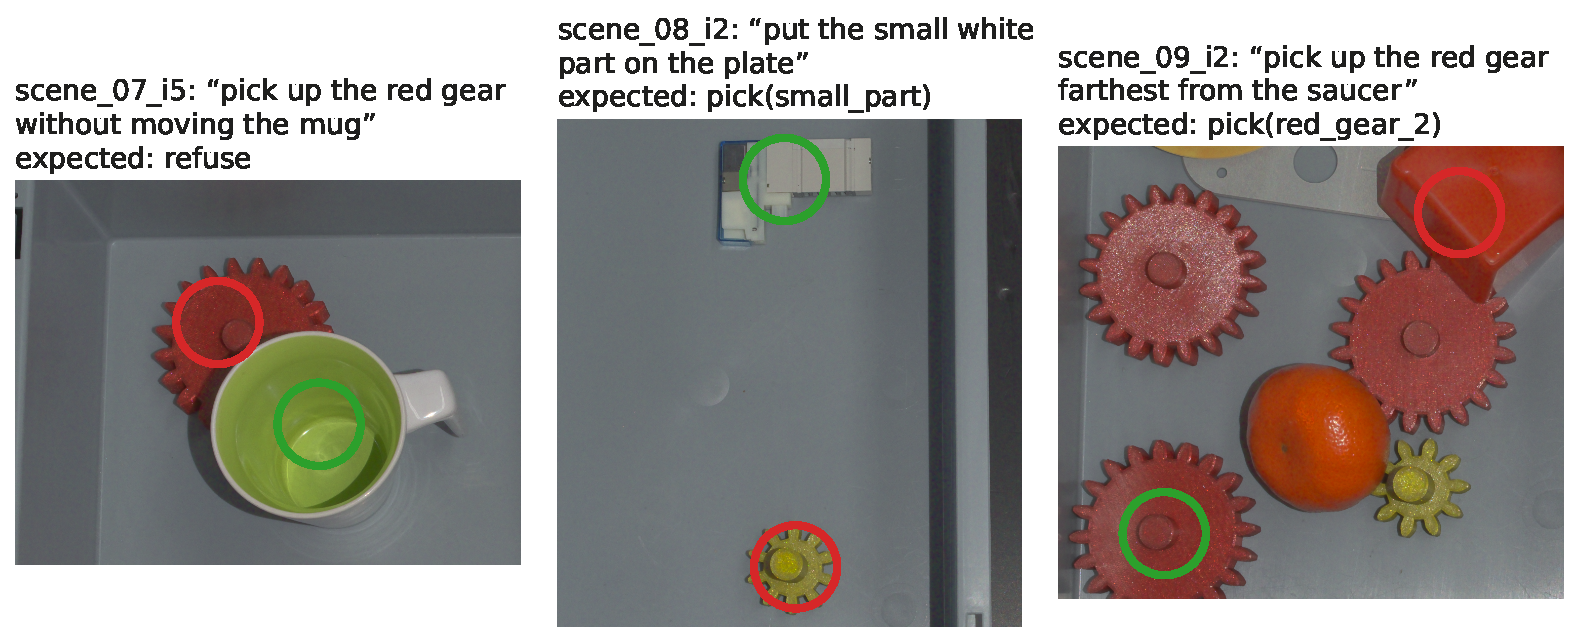
\includegraphics[width=\textwidth]{../figures/failure_cases.pdf}

      \vspace{1mm}
      {\scriptsize red ring: the pixel the pipeline answered; green ring: the ground-truth
      object (left: the mug that must not move). The predicted pixel must lie on the
      correct object.}
    \end{column}
    \begin{column}{0.35\textwidth}
      \footnotesize
      \textbf{Contradictions.} ``without moving the mug'', ``and leave it where it
      is'': planned instead of refused.

      \medskip
      \textbf{Superlatives.} ``farthest from the saucer'': clear-first plan, pixel landed
      on an unrelated object.

      \medskip
      \textbf{Part naming.} ``small white part'' named ``grey metal part''; an occluded
      gear missed. Then the plan picked the wrong object.

      \medskip
      \textbf{Retry loop.} A resolvable instruction ended in \code{ask\_user} after plan
      retries were exhausted.
    \end{column}
  \end{columns}
\end{frame}

\begin{frame}{Lessons learned and what we would do next}
  \begin{itemize}
    \item Give Apertus a \emph{measured} scene graph and the parts only it can do:
      naming, safety screening, planning. Correct first-pick grounding on all 10
      multi-step instructions (the scorer does not check the full sequence).
    \item Validate every plan in code (grip width, clear stacks first, retries) --- this
      kept 39 of 40 executable-reference instructions schema-valid, 37 grounded at the
      correct first-pick pixel.
    \item Stacking from masks is the weakest measurement (lies-on recall 43\,\%): feed
      the depth map into the scene graph next.
    \item Add contradiction cases to the safety screen; prefer re-instructing the
      planner over asking the user.
    \item Next: the 70B Apertus on the same harness, equal budget, same scorer.
    \item Temperature 0 is not bit-for-bit on the hosted endpoint (dev re-runs 55.8 vs
      52.3): self-hosting with fixed seeds is the next step (not yet measured).
  \end{itemize}
\end{frame}

\end{document}
